\section{Physical model}

\begin{frame}{Physical setup}
  \begin{itemize}
    \item A vehicle (mass $m$) rides at constant speed $v$ over a bumpy road.
    \item Road height $h(x)$ varies with distance $x$ along the road.
    \item The suspension is modeled as a mass--spring--damper system.
    \item We compute the vertical displacement $u(t)$ of the vehicle.
  \end{itemize}
  \vspace{0.4em}
  \begin{center}
    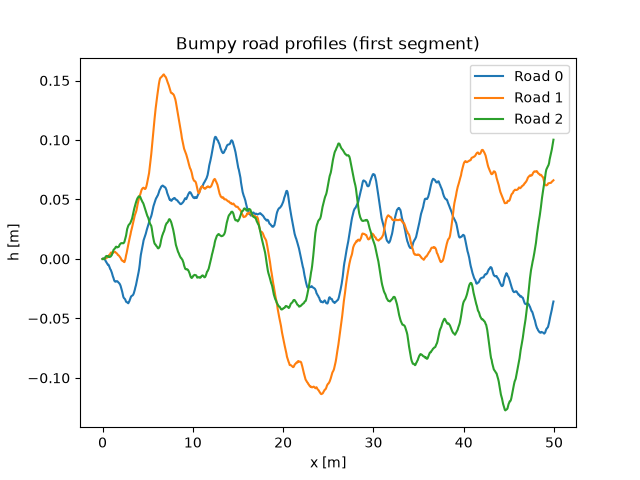
\includegraphics[width=0.48\textwidth]{figures/road_profiles.png}
  \end{center}
\end{frame}

\begin{frame}{Mathematical model}
  General vibration ODE:
  \[
  m u'' + f(u') + s(u) = F(t),
  \qquad u(0)=I,\quad u'(0)=V.
  \]
  \begin{itemize}
    \item Input: mass $m$, damping force $f(u')$, spring force $s(u)$,
          external force $F(t)$, initial data $I$, $V$
    \item Output: vertical displacement $u(t)$
  \end{itemize}
\end{frame}

\begin{frame}{Specialization used in the app}
  In \texttt{bumpy.py} we usually take
  \textbf{linear} spring and damper:
  \[
  m u'' + b u' + k u = F(t).
  \]
  \begin{itemize}
    \item $k$: spring stiffness
    \item $b$: damping coefficient
    \item Typical bicycle defaults:
          $m=60\,\mathrm{kg}$, $k=60\,\mathrm{N/m}$,
          $b=80\,\mathrm{Ns/m}$, $v=5\,\mathrm{m/s}$
  \end{itemize}
  The solver also supports \emph{quadratic} damping
  $f(u') = b|u'|u'$ (see next section).
\end{frame}

\begin{frame}{From road height to forcing}
  Constant speed: $x = v\,t$.
  Vertical acceleration of the road contact:
  \[
  a(t) = \frac{d^2}{dt^2} h(x)
       = v^2\, h''(x).
  \]
  Force on the mass:
  \[
  F(t) = -m\, a(t) = -m\, v^2\, h''(x).
  \]
  So the road curvature (and speed) set the excitation of the suspension.
\end{frame}

\begin{frame}{Animation of the ride}
  \begin{center}
    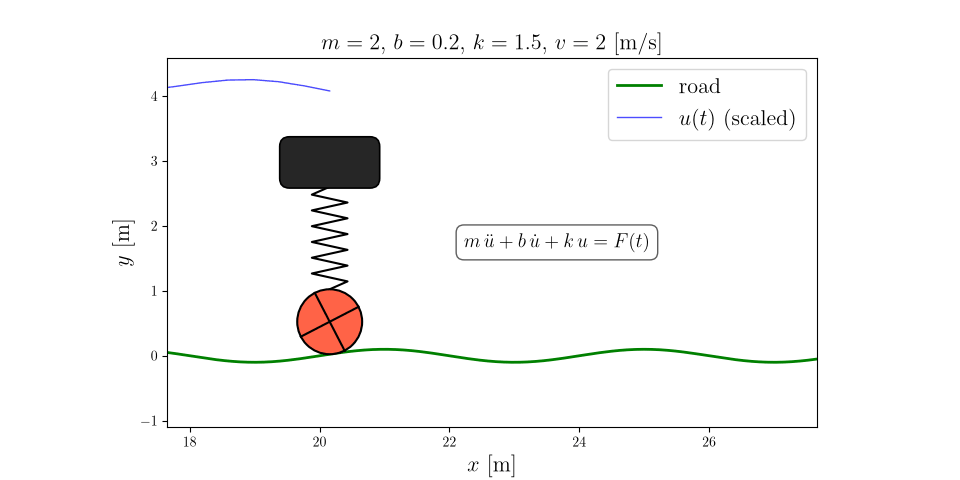
\includegraphics[width=0.75\textwidth]{figures/bumpy_road_still.png}
  \end{center}
  \vspace{0.4em}
  Snapshot from \texttt{bumpy\_road\_anim.py}
  (writes \texttt{bumpy\_road.gif} / \texttt{.mp4} in \texttt{bumpy\_road/}).
\end{frame}
